\chapter{Application I: Electric and Space Propulsion}
\label{ch:ep}

Electric propulsion (EP) is the domain in which the ion-energy-flux framework developed in earlier chapters finds its most immediate, commercially consequential deployment. Hall-effect and gridded ion thrusters are, at their core, engineered plasma sheaths: the physics governing how many ions strike a channel wall or acceleration grid, at what energy and angle, simultaneously governs how long the device survives and how efficiently it converts power into thrust. Sputtering erosion of these surfaces is the dominant life-limiting mechanism in nearly every flight-qualified EP family, and qualification campaigns built to bound it consume a disproportionate share of a programme's schedule and budget. This chapter develops the physical basis of Hall and gridded ion thrusters, shows how sheath structure governs the ion energy flux incident on erodible surfaces, reviews present diagnostics for characterising that flux and the erosion it produces, and argues that a compact, in-situ ion-energy-flux sensor closes a specific gap in thruster qualification, before turning to the commercial landscape and a plausible adoption pathway.

\section{Principles of Hall-Effect and Gridded Ion Thrusters}
\label{sec:ep-principles}

\subsection{Hall-effect thrusters: crossed-field acceleration}

A Hall-effect thruster (HET) is an annular plasma accelerator in which a radial magnetic field $B_r$ is superposed on an axial electric field $E_z$ between an upstream anode and a downstream cathode-neutralizer. Cathode electrons, magnetized by $B_r$, undergo an azimuthal $\mathbf{E}\times\mathbf{B}$ drift that closes a Hall current and greatly reduces axial electron mobility, so the applied potential drop is supported almost entirely within the channel. Neutral propellant, typically xenon, is ionized by electron-impact collisions in the dense electron layer, and the resulting ions — effectively unmagnetized, since their Larmor radius vastly exceeds the channel dimensions — are accelerated directly by the axial field, exiting as a quasi-collimated beam neutralized by cathode electrons \cite{ref0115}. No physical grid intercepts the beam: acceleration occurs in the quasi-neutral plasma itself, over a zone set by magnetic topology, propellant flow, and discharge voltage. This permits higher current densities than gridded (space-charge-limited) designs, at the cost of exposing channel walls directly to the energetic plasma producing thrust.

The discharge channel is bounded, in most flight designs, by boron-nitride ceramic walls; magnetically shielded variants configure the field so lines run nearly parallel to the walls near the exit plane, suppressing normal ion flux. Radial plasma transport to the walls, and near-wall conductivity from secondary electron emission (SEE), couples directly to axial electron transport governing discharge efficiency \cite{ref0425}, so wall interaction is integral to discharge physics, not an erosion nuisance alone.

\subsection{Gridded ion thrusters}

A gridded (electrostatic) ion thruster separates ionization and acceleration spatially. Propellant is ionized in an upstream discharge chamber — by DC discharge, RF inductive coupling, or microwave ECR heating — producing a quasi-neutral plasma bounded by closely spaced, biased grids: a screen grid near plasma potential and a downstream accelerator grid at large negative potential. Ions are extracted through aligned apertures and accelerated across the inter-grid gap, exiting as many parallel beamlets \cite{ref0115}. Because extraction current is limited by the space charge across the narrow gap, gridded thrusters run at lower current density but higher specific impulse than Hall thrusters for comparable power.

The ion-optics system generalizes the planar Child-Langmuir sheath problem treated earlier: each aperture is a miniature space-charge-limited diode, its beamlet shaped by the local plasma meniscus and radial fields at the edges. Neutral propellant escaping ionization is ionized downstream of the screen grid by charge-exchange (CEX) collisions with fast beam ions, then accelerated backward by the local field and can strike the accelerator grid — the principal erosion pathway in gridded thrusters, treated in \cref{sec:erosion}.

\subsection{Propellants and performance metrics}

Xenon dominates as propellant for both families for its high atomic mass, chemical inertness, ease of high-density storage, and low first-ionization energy. Krypton has re-emerged as a lower-cost alternative for large constellations at a modest efficiency penalty; iodine and metallic propellants remain under development. Propellant choice affects erosion significantly: sputtering yield depends on ion species as well as energy, so changing propellant can shift a device outside its xenon-qualified erosion envelope.

A second erosion-relevant metric is beam charge-state composition: a non-negligible fraction of ionized propellant is doubly or triply charged, carrying proportionally larger kinetic energy for the same accelerating voltage, since energy scales with charge state $Z$ while sputtering cross-section does not — why a bulk average ion energy inferred from discharge voltage is an unreliable proxy for the erosion-driving quantity.

Thruster performance is conventionally reported through metrics the ion-energy-flux framework connects directly to sheath physics:

\begin{align}
F &= \dot m_i \, u_{\mathrm{ex}} \, \eta_{\mathrm{d}} \;+\; (p_{\mathrm{ex}} - p_{\infty})A_{\mathrm{ex}}, \label{eq:thrust} \\
I_{\mathrm{sp}} &= \frac{F}{\dot m \, g_0}, \label{eq:isp} \\
\eta_{\mathrm{T}} &= \frac{F^2}{2\,\dot m\, P_{\mathrm{in}}}, \label{eq:effT}
\end{align}

where $F$ is thrust, $\dot m_i$ and $\dot m$ are ionized and total mass flow rates, $u_{\mathrm{ex}}$ the mean exhaust velocity, $\eta_{\mathrm{d}}$ a divergence efficiency, $I_{\mathrm{sp}}$ specific impulse, $g_0$ standard gravity, and $\eta_{\mathrm{T}}$ overall thrust efficiency referenced to input power $P_{\mathrm{in}}$. Exhaust velocity is set, for a gridded thruster, by the accelerating voltage $V_{\mathrm{a}}$, $u_{\mathrm{ex}} \approx \sqrt{2eV_{\mathrm{a}}/m_i}$, and for a Hall thruster by the discharge voltage $V_{\mathrm{d}}$ integrated over the acceleration zone, $u_{\mathrm{ex}} \approx \sqrt{2eV_{\mathrm{d}}/m_i}$ — both statements about the energy an ion gains crossing a sheath, precisely what the ion-energy-flux diagnostic in this monograph measures directly rather than infers.

\begin{table}[htbp]
\centering
\caption{Representative order-of-magnitude performance ranges for flight-class Hall-effect and gridded ion thrusters; approximate technology bands, not measurements from a specific device.}
\label{tab:ep-perf}
\begin{tabular}{lcc}
\toprule
Metric & Hall-effect thruster & Gridded ion thruster \\
\midrule
Specific impulse & \SI{1200}{}--\SI{2500}{\second} & \SI{2500}{}--\SI{4500}{\second} \\
Thrust efficiency & 45\%--65\% & 60\%--75\% \\
Thrust-to-power & \SI{40}{}--\SI{60}{\milli\newton\per\kilo\watt} & \SI{25}{}--\SI{40}{\milli\newton\per\kilo\watt} \\
Discharge/accel.\ voltage & \SI{150}{}--\SI{400}{\volt} & \SI{1000}{}--\SI{3000}{\volt} \\
Beam ion energy at target & \SI{100}{}--\SI{300}{\electronvolt} & \SI{200}{}--\SI{500}{\electronvolt} (CEX) \\
\bottomrule
\end{tabular}
\end{table}

The last row anticipates the erosion discussion below: even though nominal beam energy is set by kilovolt-level voltages, the ions actually wearing the accelerator grid are the low-energy CEX population accelerated only through the local, much smaller sheath potential.

\section{Sheaths at Channel Walls and Acceleration Grids}
\label{sec:ep-sheaths}

\subsection{The channel-wall sheath of a Hall thruster}

The Hall thruster channel wall contacts a magnetized, non-equilibrium plasma whose ions arrive with a distribution of energies and angles set by the extended acceleration zone rather than a single, sharply defined presheath. The qualitative sheath structure developed earlier — a quasi-neutral presheath accelerating ions to at least the Bohm speed, followed by a thin sheath carrying most of the wall-normal potential drop — remains the correct starting point. The Bohm velocity
\begin{equation}
u_{\mathrm{B}} = \sqrt{\frac{k_{\mathrm{B}} T_{\mathrm{e}}}{m_i}},
\label{ch16-eq:bohm}
\end{equation}
sets the minimum ion speed feeding the wall sheath, and the ion flux delivered to the wall, absent strong magnetization along the wall normal, is
\begin{equation}
\Gamma_i = n_{\mathrm{i}} u_{\mathrm{B}},
\label{eq:gammai}
\end{equation}
evaluated at the sheath edge. Two complications modify this picture: the tangential wall field component requires a magnetized (Bohm–Chodura) generalization, with ions reaching the Bohm speed within a magnetic presheath scaled by the Larmor radius rather than the Debye length, governing incidence angle and sputtering yield; and the dielectric wall charges to a floating potential set by zero net current, with SEE feeding back on the sheath drop and partially collapsing it in the saturated regime.

The sheath potential drop $\Delta\phi_{\mathrm{sh}}$ between the quasi-neutral plasma and a floating dielectric wall, neglecting SEE for a first estimate, follows
\begin{equation}
\Delta\phi_{\mathrm{sh}} = \frac{k_{\mathrm{B}} T_{\mathrm{e}}}{e}\ln\!\left(\sqrt{\frac{m_i}{2\pi m_{\mathrm{e}}}}\right),
\label{eq:floatpot}
\end{equation}
which for a xenon plasma with $T_{\mathrm{e}}\sim\SI{20}{\electronvolt}$, typical near the wall in the acceleration zone, gives a floating drop on the order of 100~V — small compared to the discharge voltage but not negligible against sputtering thresholds \cite{ref0425}. Because the acceleration zone shifts with discharge conditions and channel widening, the wall-normal ion energy flux evolves over thruster life, which in-situ measurement should track.

\subsection{The acceleration-grid sheath of a gridded ion thruster}

The grid system of a gridded ion thruster is a deliberately engineered, high-voltage space-charge-limited sheath. Ions are extracted across a vacuum gap $d$ under applied potential $V_{\mathrm{a}}$, with transmissible current density bounded by the planar Child–Langmuir law,
\begin{equation}
J_{\mathrm{CL}} = \frac{4}{9}\,\varepsilon_0 \sqrt{\frac{2e}{m_i}}\; \frac{V_{\mathrm{a}}^{3/2}}{d^2},
\label{ch16-eq:childlangmuir}
\end{equation}
which, with aperture geometry and local plasma density at the screen grid, sets the maximum extractable beam current for given voltage and gap. \Cref{ch16-eq:childlangmuir} generalizes the planar high-voltage sheath solution derived earlier, restricted to the collisionless, non-neutral inter-grid vacuum region; departures from idealized planar geometry are captured by perveance-per-hole formulations and trajectory codes, but \cref{ch16-eq:childlangmuir} remains the organizing relation for ion-optics design.

The erosion-relevant sheath is not this main accelerating sheath, which beam ions cross once and depart at high energy without striking the grids. It is instead the local sheath around the downstream accelerator-grid surfaces that responds to the CEX population: neutral propellant and beam ions undergoing charge exchange in the inter-grid gap produce slow ions accelerated back toward the accelerator grid. This local sheath structure — not the full net accelerating voltage — sets the impact energy of the eroding population \cite{ref0463}. Because this potential is typically only a few hundred volts rather than the full multi-kilovolt beam voltage, the resulting flux lands where sputtering yields for common grid materials rise steeply, making this modest-energy population the dominant erosive agent.

\subsection{Ion energy flux: the common thread}

In both architectures the erosion-relevant quantity is neither ion flux nor sheath voltage alone but their product integrated over the local energy distribution $f_{\mathrm{i}}(v)$ at the surface:
\begin{equation}
\Gamma_{E} = \int_0^{\infty} \tfrac{1}{2} m_i v^2 \, f_{\mathrm{i}}(v)\, v \, \mathrm{d}v \;\cos\theta,
\label{ch16-eq:gammaE}
\end{equation}
where $\theta$ is the angle between local ion velocity and surface normal. This is the physically correct erosion driver because sputtering yield is energy- and angle-dependent: two distributions with the same total flux $\Gamma_i = \int f_{\mathrm{i}}(v)\, v\, \mathrm{d}v$ but different energy spread produce different erosion rates — the case, developed in \cref{sec:enabling}, for measuring $\Gamma_{E}$ directly rather than inferring it from bulk parameters.

\section{Erosion as the Dominant Life-Limiting Mechanism}
\label{sec:erosion}

\subsection{Sputtering physics at the wall and grid}

Physical sputtering — ejection of surface atoms following momentum transfer from an incident ion — underlies essentially all electric-thruster erosion \cite{ref0143}. The sputtering yield $Y(E,\theta)$, the mean number of atoms ejected per incident ion, is strongly nonlinear in energy $E$: it vanishes below a threshold $E_{\mathrm{th}}$ set by surface binding energy and rises as a power law before saturating at high energies \cite{ref0152}. A widely used semi-empirical (Bohdansky/Yamamura-family) parameterization captures this behaviour:
\begin{equation}
Y(E) = A\left(\sqrt{E} - \sqrt{E_{\mathrm{th}}}\right), \qquad E \geq E_{\mathrm{th}},
\label{eq:sputterY}
\end{equation}
with $A$ a material- and species-dependent constant absorbing the nuclear stopping cross-section and surface binding energy — illustrating why erosion is so sensitive to ion energy, and why in-situ measurement of the energy distribution at the eroding surface is valuable.

\begin{figure}[htbp]
\centering
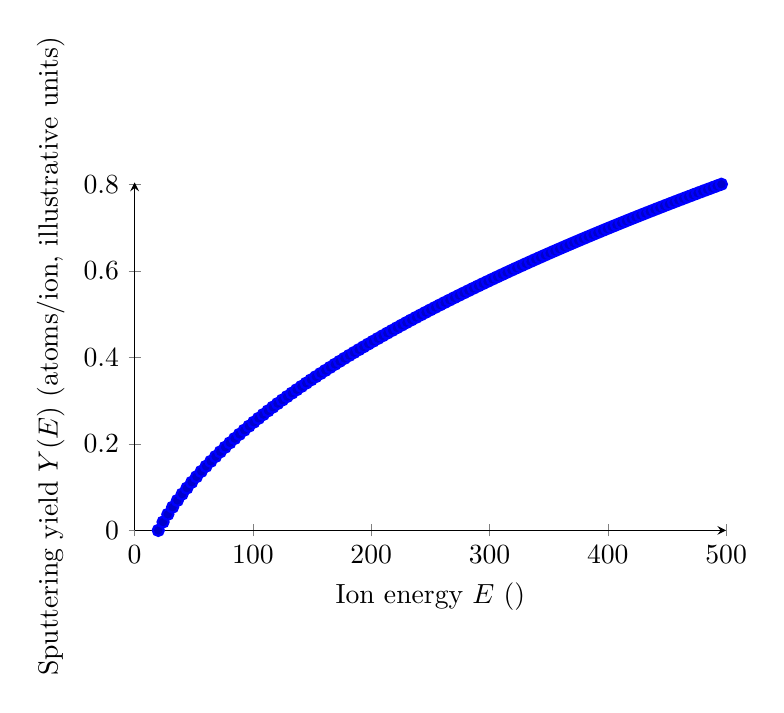
\begin{tikzpicture}
\begin{axis}[
 width=0.75\linewidth,
 height=6cm,
 xlabel={Ion energy $E$ (\si{\electronvolt})},
 ylabel={Sputtering yield $Y(E)$ (atoms/ion, illustrative units)},
 domain=20:500,
 samples=120,
 axis lines=left,
 every axis plot/.append style={thick, black},
 xmin=0, xmax=500,
 ymin=0,
]
\addplot {0.045*(sqrt(x)-sqrt(20))};
\end{axis}
\end{tikzpicture}
\caption{Schematic, illustrative sputtering-yield curve of the threshold form in \cref{eq:sputterY}, with an arbitrarily chosen threshold energy $E_{\mathrm{th}}=\SI{20}{\electronvolt}$ and prefactor $A$; a qualitative analytic model, not measured or fitted data for any specific ion-target combination.}
\label{fig:sputterY}
\end{figure}

\Cref{fig:sputterY} shows why a shift of only a few tens of volts in the characteristic energy of the erosive population — the size of the sheath potentials in \cref{sec:ep-sheaths} — can change local erosion rate by a large multiplicative factor, since most thruster erosion operates on the steep part of the yield curve, a nonlinearity that makes erosion highly sensitive to sheath-structure details with comparatively modest effect on bulk metrics such as thrust and $I_{sp}$.

\subsection{Hall thruster channel-wall erosion}

In a conventional (unshielded) Hall thruster, the ion energy flux delivered to the ceramic channel wall by \cref{ch16-eq:gammaE} directly erodes the wall, progressively widening the channel, altering the magnetic topology, and ultimately exposing the pole pieces or distorting the discharge \cite{ref0425}. This erosion is not spatially uniform: the acceleration zone, where ion energy is highest, produces the most aggressive local erosion, and the profile evolves as channel geometry changes and shifts the zone — a self-modifying feedback loop that makes early-life extrapolation unreliable unless the underlying flux, not just resulting recession, is tracked \cite{ref0433}. If ions of energy $E$ each remove, on average, $Y(E)$ target atoms, the recession rate normal to the surface is
\begin{equation}
\dot h = \frac{M}{\rho N_{\mathrm{A}}} \int_0^{\infty} Y\!\left(\tfrac{1}{2}m_i v^2\right) f_{\mathrm{i}}(v)\, v\, \mathrm{d}v\, \cos\theta,
\label{eq:erosionrate}
\end{equation}
where $M$ is the wall material's molar mass, $\rho$ its density, and $N_{\mathrm{A}}$ the Avogadro constant. \Cref{eq:erosionrate} makes explicit that erosion rate is not proportional to $\Gamma_{E}$ of \cref{ch16-eq:gammaE}, since $Y(E)$ is energy-dependent and convex; a full accounting requires $f_{\mathrm{i}}(v)$, not merely its second moment.

Life testing has repeatedly shown channel-wall erosion to be historically the pacing item for Hall thruster qualified life in unshielded designs, motivating witness-coating measurement and predictive modelling with hybrid fluid-PIC and kinetic codes to extrapolate short-duration data to multi-year life \cite{ref0433,ref0440}. Magnetic shielding, reshaping field topology so lines run tangential to the wall, was a direct engineering response: reducing wall-normal flux can extend qualified life by an order of magnitude, at the cost of exposing pole covers to a residual flux that must itself be characterized.

\subsection{Grid erosion: pits-and-grooves and accelerator-grid wear-out}

Gridded ion thrusters exhibit a qualitatively distinct erosion signature dominated by CEX-ion bombardment of the accelerator grid, producing two characteristic wear patterns. Pits-and-grooves erosion arises from CEX ions accelerated back through the local sheath and focused by residual field structure onto the downstream grid face, eroding grooves connecting adjacent apertures at end of life. Chamfer (barrel) erosion of the aperture walls is caused by CEX ions born within the gap striking the inner wall at grazing incidence, progressively enlarging the aperture until perveance and structural margin are compromised. Both mechanisms are quantitatively predicted using hybrid CEX-tracking codes (the CEX2D/CEX3D lineage) coupling beam-ion trajectories to a Monte Carlo charge-exchange model and a yield-based update \cite{ref0463}, validated against long-duration wear tests \cite{ref0480}.

Facility background pressure is a first-order confound in ground-based grid erosion testing: elevated neutral density relative to the true space environment increases CEX production above flight-representative levels, so facility-induced erosion can substantially overstate the true in-orbit rate unless corrected \cite{ref0461,ref0481}, arguing for a diagnostic that distinguishes the CEX-driven component from the flight-representative beam-driven one in situ.

\subsection{Qualification needs}

Flight qualification of an EP thruster requires demonstrating, with adequate margin, that erosion accumulated over the full mission — commonly many thousands of hours, and for large GEO or deep-space platforms tens of thousands — will not compromise structural integrity or discharge stability. Because full-duration life testing at the actual throttle profile is prohibitively expensive (a \SI{10000}{\hour} test is well over a year of operation), qualification programmes rely on partial-duration wear tests extrapolated using validated erosion models and post-test destructive metrology. Each shares a limitation: erosion is characterized after the fact, at coarse temporal resolution, with the underlying flux inferred rather than measured directly. A diagnostic tracking flux to the eroding surface throughout a wear test would let erosion models be validated near-real time, shortening the campaign and providing grounded uncertainty bounds on extrapolated margins \cite{ref0440}.

Qualification practice further complicates the picture through accelerated throttle points, where a thruster is operated above nominal voltage or current to compress a multi-year erosion accumulation into a shorter test duration. Because the yield in \cref{eq:sputterY} is convex and nonlinear, accelerated-life data cannot be linearly rescaled to the nominal throttle point without a validated mapping; an erosion rate measured at elevated voltage overstates the nominal rate by a factor set by the local slope of $Y(E)$ — information a continuous, in-situ measurement supplies and a bulk setpoint does not.

\section{Existing Diagnostics and Their In-Situ Shortcomings}
\label{sec:ep-diagnostics}

\subsection{Ex-situ and post-test erosion metrology}

The most direct and widely trusted erosion measurement remains post-test physical metrology: profilometry, laser triangulation, or optical microscopy of channel-wall or grid geometry before and after a wear-test segment, giving an interpretable recession depth at high resolution. Multilayer witness coatings, with erosion depth read out from the exposed-layer sequence, extend this to intermediate checkpoints without full disassembly. These methods remain, especially for grid geometry, the standard against which erosion models are validated \cite{ref0480}. Their shortcoming is temporal: the thruster must be shut down and accessed with dedicated instrumentation, so erosion is measured only at discrete milestones separated by tens to hundreds of operating hours, during which the plasma conditions actually driving erosion go uncharacterized. A cumulative depth measured at interval's end cannot distinguish a steady low-level rate from a short-duration high-rate excursion.

\subsection{In-situ optical and plasma diagnostics}

A substantial body of in-situ technique characterizes the plasma conditions driving erosion without interrupting operation. Laser-induced fluorescence (LIF), resolving the ion velocity distribution function along a line of sight, has been used extensively in Hall thruster channels and plumes to measure ion velocity and energy versus axial position, evidencing the acceleration zone's location and shift over life \cite{ref0322,ref0347}. Optical emission spectroscopy (OES) of sputtered material and emission-line ratios has similarly served as an indirect, real-time erosion-rate proxy \cite{ref0257}. Electrostatic and emissive probes provide local density, temperature, and plasma-potential measurements that, with a Bohm-criterion closure, estimate ion flux and energy at a location \cite{ref0226,ref0490}. Thomson scattering provides non-perturbing density and temperature measurements, and with sufficient resolution ion properties, inside the channel \cite{ref0356}. Momentum-flux instruments give an integral measure of exhaust momentum that constrains but does not resolve the underlying flux \cite{ref0511}.

\subsection{The diagnostic gap}

Despite this rich toolkit, a specific gap persists between what these instruments measure and what erosion modelling in \cref{eq:erosionrate} actually requires: a directly measured, energy-resolved ion flux $f_{\mathrm{i}}(v)$, or at minimum its moment $\Gamma_{E}$, sampled continuously and non-destructively at the erodible surface. Several structural limitations explain why this gap persists:

\begin{itemize}
\item \textbf{Optical line-of-sight access.} LIF and OES require unobstructed optical access; near the channel wall or a grid aperture, occlusion and window fouling from sputtered material degrade signal quality precisely as a campaign approaches end-of-life \cite{ref0454}.
\item \textbf{Perturbation by physical probes.} Probes close enough to sample the sheath-edge population necessarily perturb what they measure, and probe survivability in the high-flux region is limited by the same sputtering physics driving the erosion of interest.
\item \textbf{Indirect inference chains.} Bulk measurements away from the eroding surface must be propagated to the wall or grid through a presheath/sheath model, introducing uncertainty exactly where energy resolution matters most \cite{ref0425}.
\item \textbf{Post-test-only ground truth.} Erosion-rate proxies (OES, witness coatings) measure the erosion consequence, not the causative flux, so they validate an integrated rate but cannot discriminate models predicting the same erosion from different energy distributions \cite{ref0454}.
\item \textbf{Facility-environment conflation.} Ground-test background pressure elevates CEX production above flight-representative levels, so diagnostics measuring only the resulting erosion rate cannot separate the facility artefact from the flight signal \cite{ref0461,ref0481}.
\end{itemize}

\begin{table}[htbp]
\centering
\caption{Qualitative comparison of existing diagnostic approaches against the requirement of continuous, in-situ, energy-resolved ion flux measurement at the erodible surface. Entries reflect general characteristics discussed in the cited literature, not a specific instrument.}
\label{tab:diagcompare}
\begin{tabularx}{\linewidth}{lXcc}
\toprule
Technique & Primary observable & Continuous in-situ? & Energy-resolved at wall/grid? \\
\midrule
Post-test profilometry / metrology & Cumulative recession depth & No & No \\
Multilayer witness coatings & Cumulative recession depth & Milestone-only & No \\
Laser-induced fluorescence & Ion velocity along line of sight & Yes, with access & Partial (indirect) \\
Optical emission spectroscopy & Line intensity ratios, $T_{\mathrm{e}}$ proxy & Yes & No \\
Electrostatic / emissive probes & $n_{\mathrm{e}}$, $T_{\mathrm{e}}$, plasma potential & Perturbative, local & Indirect via closure \\
Thomson scattering & $n_{\mathrm{e}}$, $T_{\mathrm{e}}$ (bulk) & Yes, complex setup & No \\
\bottomrule
\end{tabularx}
\end{table}

\Cref{tab:diagcompare} summarizes the pattern: no diagnostic in routine use today combines continuous operation, in-situ deployment at the erosion-relevant surface, and direct energy resolution. Existing techniques either resolve energy (LIF, probes) at the cost of continuous or non-perturbing operation, or provide continuous erosion-relevant signals (OES, witness coatings) at the cost of energy resolution, forcing modellers to bridge the gap with sheath-closure assumptions that remain the weakest link in current lifetime prediction.

\section{How the Framework Enables Lifetime Prediction and Design Optimization}
\label{sec:enabling}

\subsection{From ion energy flux to erosion-rate closure}

The kinetic sheath and presheath theory developed earlier provides the missing closure between an in-situ measurement of $f_{\mathrm{i}}(v)$, or its low-order moments $\Gamma_i$ and $\Gamma_{E}$, at an accessible location near — but not necessarily at — the erodible surface, and the flux-and-energy pair actually incident on it. Because the sheath is thin compared to device scale, and the kinetic Bohm criterion fixes the minimum ion speed entering the sheath as a function of $T_{\mathrm{e}}$ alone, a measurement of $n_{\mathrm{i}}$, $T_{\mathrm{e}}$, and sheath-edge distribution shape can be propagated through the collisionless sheath solution to the wall with far lower uncertainty than propagating a bulk-plasma measurement through both regions — converting an accessible measurement into a wall-normal flux estimate, insertable into \cref{eq:erosionrate} to produce a predicted local erosion rate.

\subsection{Design optimization loop}

Coupling an in-situ ion-energy-flux measurement to the erosion-rate closure of \cref{eq:erosionrate} closes a design-optimization loop currently open in practice. In present workflows, a candidate magnetic-field topology, channel geometry, or grid-gap design is evaluated primarily through simulation \cite{ref0433,ref0463}, validated only at coarse post-test resolution, and discrepancies are diagnosed by re-running the simulation with adjusted parameters, since the actual flux delivered to the wall was never independently measured. An in-situ sensor breaks this circularity, supplying an independent, time-resolved measurement of the very quantity the simulation is trying to predict — particularly valuable for magnetically shielded designs, where confirming reduced wall-normal flux in situ would de-risk the shielding process relative to cumulative pole-erosion measurements alone.

\subsection{Lifetime extrapolation and digital-twin qualification}

Perhaps the most consequential application is lifetime extrapolation itself. Because $\dot h$ in \cref{eq:erosionrate} depends nonlinearly on the ion energy distribution through $Y(E)$, and that distribution evolves over operating life as channel or grid geometry changes, a lifetime model anchored to periodic, in-situ measurements can track this evolution and update its extrapolated end-of-life margin continuously, rather than only at the single checkpoints presently used \cite{ref0440}. This supports a digital-twin paradigm: a reduced-order erosion model, already used for Hall thruster lifetime prediction \cite{ref0433}, is continuously re-anchored against a live signal rather than validated once and trusted to extrapolate unchecked. For gridded thrusters, the same principle separates flight-representative beam-driven wear from facility-pressure-driven CEX wear, potentially shortening the multi-thousand-hour tests required to bound facility uncertainty \cite{ref0461,ref0481}, and offers a route to qualifying new propellants against a physically grounded model.

\section{Market Context and Adoption Pathway}
\label{sec:ep-market}

\subsection{Commercial and institutional landscape}

Electric propulsion has moved, over roughly two decades, from a niche technology on a handful of GEO and deep-space missions to a mainstream choice across the commercial and institutional spacecraft market. Large LEO broadband constellations use Hall-effect thrusters for orbit raising, station-keeping, collision avoidance, and controlled deorbit, prizing low per-unit cost and qualified life for a multi-year, high-duty-cycle lifetime. GEO operators have adopted all-electric or hybrid-electric buses to cut launch mass by replacing chemical station-keeping and, in some cases, orbit-raising propellant, trading launch-cost savings against qualified thruster life. Deep-space missions rely on gridded ion thrusters, prized for high specific impulse, where mission $\Delta v$ is large and flight duration is years, so propellant-mass savings from high $I_{\mathrm{sp}}$ dominate the trade even at low thrust \cite{ref0115}. Across these segments, qualified thruster life and the confidence with which it can be predicted are recurring gating items in mission design and insurance underwriting: a thruster whose qualified life carries a wide, empirically derived uncertainty band is priced less favourably than one backed by a continuously validated erosion model.

Beyond the established industrial base, small-satellite and in-space servicing companies are developing lower-power electric thrusters for smallsats, cislunar tugs, and orbital transfer vehicles — a segment more exposed to the cost and schedule burden of erosion qualification since it cannot amortize a full-duration test across as large a production run.

\subsection{Value proposition of an in-situ ion-energy-flux sensor}

Set against this landscape, a compact, in-situ ion-energy-flux sensor addresses a specific, recurring cost driver: the schedule and budget consumed by erosion qualification, and the residual uncertainty in end-of-life margin after testing completes. The value proposition operates on three axes: schedule compression, since continuous erosion-rate tracking lets model-based extrapolation substitute for a portion of full-duration testing; margin credibility, since an independently measured flux, propagated through a validated sheath closure, gives reviewers and insurers a physically traceable basis for accepting an extrapolated margin rather than relying solely on simulation; and design iteration speed, since the sensor reads directly on the quantity magnetic shielding and grid-geometry changes are intended to control, shortening the design-test-redesign cycle for longer-life variants.

\subsection{Adoption pathway}

A realistic adoption pathway follows the standard technology-readiness progression familiar to the EP community. At the laboratory validation stage, the sensor is demonstrated on a ground-test thruster of known erosion behaviour, cross-validated against the suite of \cref{sec:ep-diagnostics} — LIF, post-test metrology, witness coatings — to establish fidelity and uncertainty bounds \cite{ref0454,ref0490}. At the qualification-support stage, it is integrated into an existing wear-test campaign as a supplementary diagnostic, correlating its signal with conventional milestone measurements \cite{ref0490,ref0511}. At the design-tool integration stage, its output is coupled into the workflow of \cref{sec:enabling}, first for design iteration and, as confidence accumulates, as evidence in qualification packages. Finally, at the flight-heritage stage, a radiation-tolerant derivative becomes a candidate for an in-flight diagnostic package, of the kind already flown to monitor thruster health and plume interaction \cite{ref0496}.

Each stage is deliberately incremental: the sensor is a complement to, not a replacement for, the established toolkit, entering as an independent cross-check and only progressively as a primary input to erosion-life certification.

\section{Summary}

Hall-effect and gridded ion thrusters are, from a plasma-physics standpoint, engineered exploitations of the sheath and presheath structures analysed throughout this monograph: thrust and specific impulse are set by the energy ions gain crossing an acceleration structure, while erosion — the dominant life-limiting mechanism in both architectures — is set by the same ion population's energy flux onto the channel wall or grid, filtered through a strongly nonlinear sputtering yield. This chapter has shown that the ion energy flux $\Gamma_{E}$, and the full distribution $f_{\mathrm{i}}(v)$ at the erodible surface, is the physically correct and currently under-measured quantity linking sheath physics to erosion rate, and that existing diagnostics each capture only part of this picture, with none combining continuous, in-situ, energy-resolved measurement at the surface itself. The sheath-transition theory developed earlier supplies the closure needed to propagate an accessible measurement to a wall-normal erosion-rate prediction with a grounded uncertainty budget, enabling a closed design-optimization loop, continuously re-anchored lifetime extrapolation, and a defensible route to shortening qualification campaigns. Against a commercial landscape where qualified-life uncertainty remains a recurring cost driver, an in-situ ion-energy-flux sensor represents a targeted, incrementally adoptable instrument with a clear rationale and a plausible pathway to flight heritage.
